\documentclass[a4paper,fleqn]{cas-dc}
\usepackage[T1]{fontenc}
\usepackage{microtype}
\usepackage{graphicx}
\usepackage{booktabs}
\usepackage{multirow}
\usepackage{amsmath}
\usepackage{array}
\usepackage{float}
\usepackage{enumitem}
\usepackage{natbib}
\usepackage{url}
\emergencystretch=3em
\setlength{\tabcolsep}{4pt}

\begin{document}
\let\WriteBookmarks\relax

\shorttitle{Hybrid Plant Disease Classification}
\title[mode=title]{A Hybrid Deep Learning Framework for Multi-Crop Plant Disease Classification Using Strategic Data Augmentation}

\author[1]{Author Name}
\ead{author@iiitp.ac.in}
\author[1]{Anupama Arun}
\ead{anupamaarun21@cse.iiitp.ac.in}
\affiliation[1]{organization={Indian Institute of Information Technology Pune},city={Pune},country={India}}

\begin{abstract}
Plant disease recognition from images can support scalable crop monitoring, but high accuracy on a single controlled dataset does not necessarily imply robustness across crops, symptom scales, or acquisition conditions. This study presents PlantDiseaseNet-Hybrid, a custom convolutional neural network designed around two complementary feature-fusion mechanisms. Parallel $3\times3$, $5\times5$, and $7\times7$ convolutional branches are fused by element-wise addition in the proposed Inception(Add) module. This keeps the branch-fusion width fixed while retaining multi-scale receptive fields. Later SkipConnection(Concat) modules concatenate transformed features with the incoming representation, explicitly retaining earlier information for subsequent classification. The design therefore uses addition for compact multi-scale integration and concatenation for feature preservation and reuse. Global average pooling is used before the dense classifier to avoid the parameter expansion associated with flattening high-resolution feature maps. The study evaluates selected PlantVillage classes, a three-class wheat disease dataset, a six-class cotton disease dataset, and an India SoyDisease dataset. A separate augmentation study evaluates several transformation policies instead of treating augmentation as an unanalysed preprocessing step. Repository-verified primary experiments record 97.81\% accuracy for wheat, 53.55\% for cotton, and 97.67\% for the selected PlantVillage experiment. On the controlled 24-class architecture comparison, the complete hybrid records 95.91\% accuracy with 934,200 total parameters, while a residual baseline records 96.04\%. The dedicated augmentation study records 97.06\% for the LightAug configuration. The strongest SoyDisease configuration records 99.44\% on its held-out evaluation and 99.57\% $\pm$ 0.85\% mean accuracy across five folds. These results support a measured conclusion: the proposed architecture is a compact dual-mode feature-fusion design rather than a model that universally dominates all baselines, and its value is best assessed through the interaction of feature fusion, parameter control, augmentation policy, and cross-crop behaviour.
\end{abstract}

\begin{keywords}
Plant disease classification \sep Hybrid CNN \sep Inception network \sep Feature fusion \sep Skip connections \sep Data augmentation \sep Agricultural computer vision
\end{keywords}
\maketitle

\section{Introduction}
Plant diseases caused by fungal, bacterial, viral, and pest-related factors can reduce crop productivity and quality. Disease diagnosis is traditionally based on visual inspection by farmers, extension personnel, or plant pathologists. Although expert assessment remains important, manual inspection is difficult to scale when large numbers of images must be processed consistently. Image-based deep learning provides a complementary approach in which discriminative representations can be learned from labelled examples.

The PlantVillage image repository and subsequent deep-learning studies established an important benchmark for image-based plant disease recognition \citep{hughes2015,mohanty2016}. Such benchmark datasets are useful because they provide controlled class labels and substantial image collections. However, controlled benchmark performance should not be interpreted automatically as field robustness. Image background, illumination, symptom severity, crop morphology, class imbalance, and acquisition conditions can alter the visual distribution presented to a classifier.

The architecture of a classifier is also important. Disease symptoms may be expressed as small lesions, elongated vein discoloration, broad colour changes, powdery regions, or pest damage. These patterns can exist at different spatial scales. Inception-style architectures address this issue through parallel convolutions with different receptive fields \citep{szegedy2015}. Standard Inception generally concatenates branch outputs. Although this preserves each branch as a separate group of channels, it also increases the channel width at the fusion point. PlantDiseaseNet-Hybrid instead adds the parallel branch outputs element-wise. This keeps the number of output channels equal to the branch width and therefore provides a direct mechanism for controlling representation growth.

Feature preservation is treated as a different problem. Residual networks use additive shortcuts to facilitate optimisation \citep{he2016}, whereas DenseNet demonstrated the value of concatenating earlier and later features to promote reuse \citep{huang2017}. The proposed SkipConnection(Concat) block adopts the latter principle locally. It retains the incoming representation while appending features learned by a $7\times7$ convolution and batch normalisation. Thus the network does not use one fusion operation everywhere. It uses \emph{addition for multi-scale branch integration} and \emph{concatenation for feature retention}. This is the dual-mode fusion principle underlying the proposed architecture.

An additional architectural revision concerns the classifier head. Earlier project implementations used a flattening operation before dense layers, producing a substantially larger parameter count. The final implementation uses global average pooling, which reduces an $H\times W\times C$ feature map to $C$ channel descriptors before the dense layers. This changes the computational role of the classifier head without changing the convolutional feature-extraction concept. The repository therefore contains different generations of the implementation, and their parameter counts are not treated as interchangeable measurements.

The study addresses four questions: (1) how does the hybrid architecture behave across crop-specific datasets; (2) what is observed when its two fusion mechanisms are isolated in controlled architecture variants; (3) which augmentation policy is most effective on the combined multi-crop setting; and (4) how does the model behave on the additional SoyDisease dataset, where the available processed subset is small and highly imbalanced? These questions are reported in separate sections to prevent dataset changes from being incorrectly described as architectural ablations.

The contributions are: (i) a custom Inception(Add)+SkipConnection(Concat) architecture; (ii) an explicit dual-mode fusion rationale; (iii) a parameter-controlled classifier head using global average pooling; (iv) crop-specific, combined, and component-level experiments; (v) a dedicated augmentation sensitivity study; and (vi) a separate SoyDisease evaluation including five-fold validation for the strongest configuration.

\section{Related Work}
Mohanty et al. demonstrated deep CNN-based plant disease classification using PlantVillage and reported the potential of image-based learning for automated diagnosis \citep{mohanty2016}. Reviews have subsequently documented the growth of CNN, transfer-learning, and explainability approaches in plant disease analysis \citep{saleem2019}. These studies motivate both strong benchmark evaluation and careful interpretation of generalisation.

Inception introduced multi-scale parallel convolutions \citep{szegedy2015}; ResNet introduced residual addition \citep{he2016}; and DenseNet introduced dense feature concatenation \citep{huang2017}. PlantDiseaseNet-Hybrid is conceptually related to all three but assigns their fusion ideas to different stages. Multi-scale branches are added to control channel growth, whereas skip features are concatenated to preserve information.

Transfer-learning comparisons show that model selection can substantially affect plant-disease classification performance \citep{too2019,atila2021}. The present study differs in that the primary contribution is a compact custom architecture rather than selection of a large pretrained backbone.

The wheat experiment uses the public three-class Wheat Disease Detection dataset associated with Safarijalal et al. \citep{safarijalal2022}. Long et al. provide a complementary field-oriented wheat study showing why realistic image variability matters for disease classification \citep{long2023}. The cotton experiment uses the six-class Cotton Plant Disease resource attributed to Dhamodharan; subsequent peer-reviewed work documents use of the same dataset \citep{cotton2024}. The SoyDisease experiment uses the India soyabean dataset of Kotwal et al. \citep{kotwal2024}.

The augmentation reporting structure is informed by Mhala et al. \citep{mhala2025}. The potato augmentation notebook present in the original project is not used as experimental evidence in this work; it is excluded from the paper-aligned experimental set.

\section{Materials and Methods}
\subsection{Datasets}
The main combined experiment contains 24 classes: 15 selected PlantVillage classes, three wheat classes, and six cotton classes. SoyDisease is not merged into this 24-class label space and is evaluated separately.

\begin{table*}[!t]
\centering
\caption{Experimental datasets and their roles.}
\label{tab:datasets}
\begin{tabular}{p{3.1cm}p{3.4cm}p{1.2cm}p{5.8cm}}
\toprule
Dataset & Role & Classes & Experimental description \\
\midrule
PlantVillage selected subset & Primary / 18-class benchmark & 15 & Bell Pepper (2), Potato (3), Tomato (10). \\
Wheat Disease Detection & Primary / 18-class benchmark & 3 & Brown Rust, Healthy, Yellow Rust. \\
Cotton Plant Disease & Primary / 24-class benchmark & 6 & Aphids, Army Worm, Bacterial Blight, Healthy, Powdery Mildew, Target Spot. \\
India SoyDisease & Separate crop study & 6 & Healthy, Vein Necrosis, Dry Leaf, Septoria Brown Spot, Root Images, Bacterial Leaf Blight. \\
\bottomrule
\end{tabular}
\end{table*}

The recorded 24-class mapping is provided explicitly below.

\begin{table*}[!t]
\centering
\caption{Complete 24-class mapping used by the combined benchmark.}
\label{tab:classes}
\begin{tabular}{rllr}
\toprule
No. & Crop & Class & Images \\
\midrule
1 & Bell Pepper & Bacterial Spot & 997 \\
2 & Bell Pepper & Healthy & 1478 \\
3 & Potato & Early Blight & 1000 \\
4 & Potato & Late Blight & 1000 \\
5 & Potato & Healthy & 152 \\
6 & Tomato & Bacterial Spot & 2127 \\
7 & Tomato & Early Blight & 1000 \\
8 & Tomato & Late Blight & 1909 \\
9 & Tomato & Leaf Mold & 952 \\
10 & Tomato & Septoria Leaf Spot & 1771 \\
11 & Tomato & Spider Mites & 1676 \\
12 & Tomato & Target Spot & 1404 \\
13 & Tomato & Yellow Leaf Curl Virus & 3209 \\
14 & Tomato & Mosaic Virus & 373 \\
15 & Tomato & Healthy & 1591 \\
16 & Wheat & Brown Rust & 902 \\
17 & Wheat & Healthy & 1116 \\
18 & Wheat & Yellow Rust & 924 \\
19 & Cotton & Aphids & 800 \\
20 & Cotton & Army Worm & 800 \\
21 & Cotton & Bacterial Blight & 800 \\
22 & Cotton & Healthy & 800 \\
23 & Cotton & Powdery Mildew & 800 \\
24 & Cotton & Target Spot & 788 \\
\midrule
\multicolumn{3}{r}{Total} & 28369 \\
\bottomrule
\end{tabular}
\end{table*}

\subsection{Preprocessing}
All model inputs are resized to $256\times256$ RGB images. Pixel values are normalised before training. The experimental record contains 2,942 wheat images, 4,788 cotton images, and 20,639 selected PlantVillage images, giving 28,369 images in the combined 24-class record. These are experimental class-selection counts and are not claims about the full size of the original public repositories.

Preprocessing is separated from augmentation. Resizing and normalisation establish a common representation; augmentation changes the training distribution and is therefore evaluated independently.

\begin{figure*}[!t]
\centering
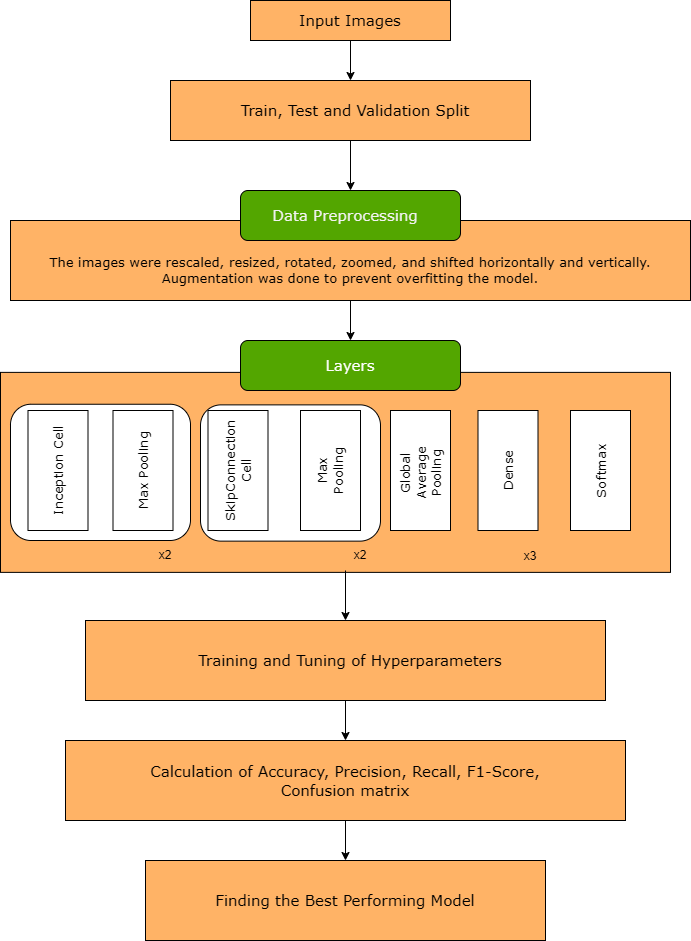
\includegraphics[width=\textwidth,height=0.36\textheight,keepaspectratio]{paper_figures/preprocessing_pipeline.png}
\caption{Preprocessing pipeline. Width and height limits are applied simultaneously to keep the complete figure within the page boundary.}
\label{fig:preprocess}
\end{figure*}

\subsection{Strategic Data Augmentation}
The project implements horizontal flipping, random rotation, zoom, brightness adjustment, translation, and contrast enhancement. These transformations target orientation, framing, illumination, and small spatial variation while attempting to preserve disease morphology.

The augmentation study is reported separately because listing transformations alone cannot establish their usefulness. Five recorded policies are compared: Hybrid-NoAug, Hybrid-LightAug, Hybrid-LightAug-v2, Hybrid-CropColour, and Hybrid-FullAug. LightAug combines horizontal flipping and brightness adjustment. The independent LightAug-v2 run provides a useful indication of run-to-run variation. FullAug represents the broader transformation set recorded by the project.

\begin{figure*}[!t]
\centering
\fbox{\parbox{0.88\textwidth}{\centering\vspace{0.2cm}\textit{FIGURE TO INSERT: VERIFIED AUGMENTATION EXAMPLES}\par\smallskip Insert the verified before/after augmentation panel and/or augmentation-policy visualisation from the executed augmentation notebooks. The figure file is not asserted here because its existence could not be independently verified from the current paper branch.\vspace{0.2cm}}}
\caption{Representative augmentation examples. The final submission should replace this placeholder with the verified augmentation figure generated by the recorded augmentation experiments.}
\label{fig:augmentation}
\end{figure*}

\subsection{PlantDiseaseNet-Hybrid Architecture}
The network accepts a $256\times256\times3$ RGB input and contains two Inception(Add) cells, four max-pooling operations, two SkipConnection(Concat) blocks, global average pooling, two dense layers, dropout, and a 24-unit softmax classifier.

The first Inception cell produces 16 channels at $256\times256$. After normalisation and pooling, the second produces 32 channels at $128\times128$. The second normalisation and pooling stage produces $64\times64\times32$. SkipConnection(Concat)-1 produces $64\times64\times96$. Pooling then produces $32\times32\times96$, and SkipConnection(Concat)-2 produces $32\times32\times224$. A fourth pooling operation produces $16\times16\times224$. Global average pooling reduces this tensor to 224 features before the dense classifier.

\begin{figure*}[!t]
\centering
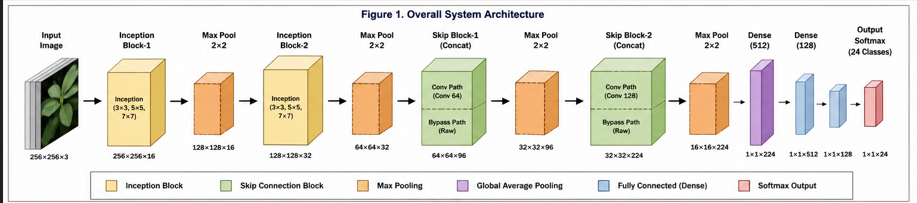
\includegraphics[width=\textwidth,height=0.42\textheight,keepaspectratio]{paper_figures/overall_architecture.png}
\caption{Overall PlantDiseaseNet-Hybrid architecture. The figure is constrained by both width and height to avoid clipping.}
\label{fig:architecture}
\end{figure*}

\subsubsection{Inception(Add)}
The three branches use $3\times3$, $5\times5$, and $7\times7$ convolutions. Their outputs are fused by
\begin{equation}
Y=F_{3\times3}(X)+F_{5\times5}(X)+F_{7\times7}(X).
\end{equation}
The branch outputs therefore do not multiply the channel dimension at the fusion point. If each branch contains $C$ channels, addition returns $C$ channels whereas concatenation would return $3C$. This is the principal computational motivation for Add fusion. The trade-off is that branch-specific responses are not retained as separate channel groups after fusion.

\begin{figure}[!t]
\centering
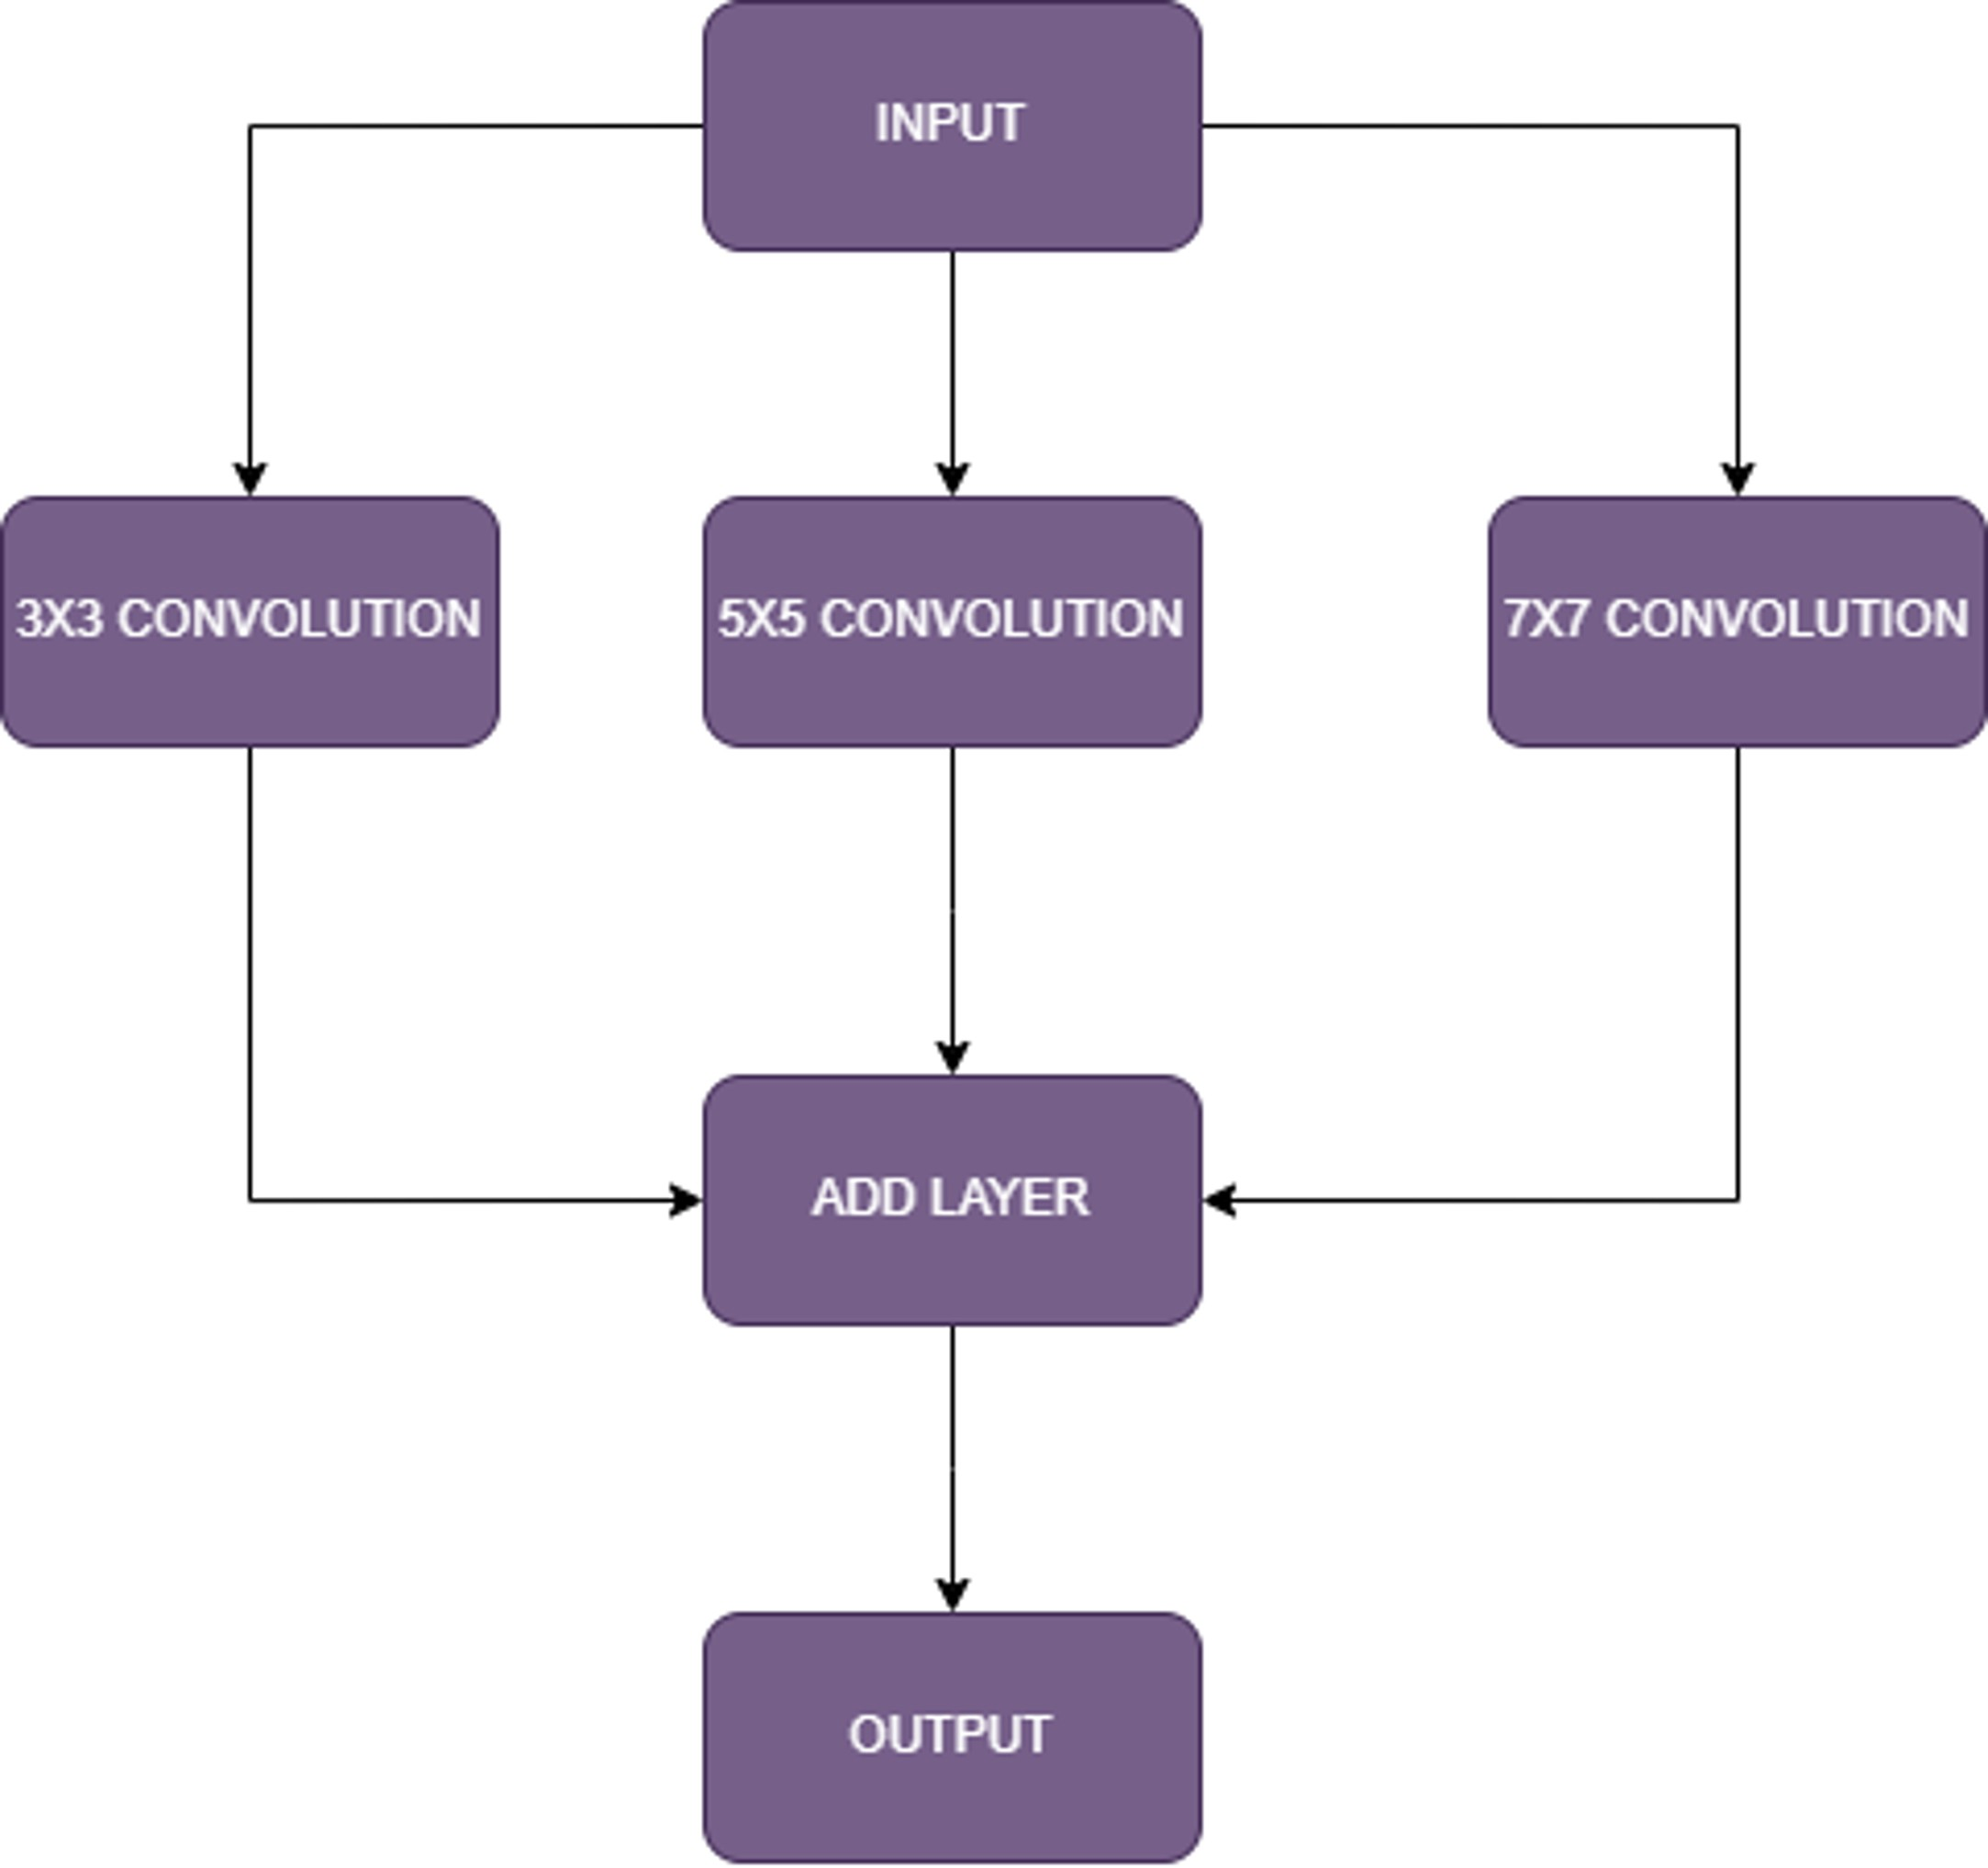
\includegraphics[width=\columnwidth,height=0.27\textheight,keepaspectratio]{paper_figures/inception_block.jpg}
\caption{Proposed Inception(Add) block.}
\label{fig:inception}
\end{figure}

\subsubsection{SkipConnection(Concat)}
The skip block applies a $7\times7$ convolution and batch normalisation and then concatenates the transformed output with the input:
\begin{equation}
Y=\operatorname{Concat}(X,F(X)).
\end{equation}
This operation retains the incoming representation and appends newly learned features. The first block expands depth from 32 to 96 channels and the second from 96 to 224. These expansions occur after spatial downsampling, making the cost more controlled than equivalent expansion at the original resolution.

\begin{figure}[!t]
\centering
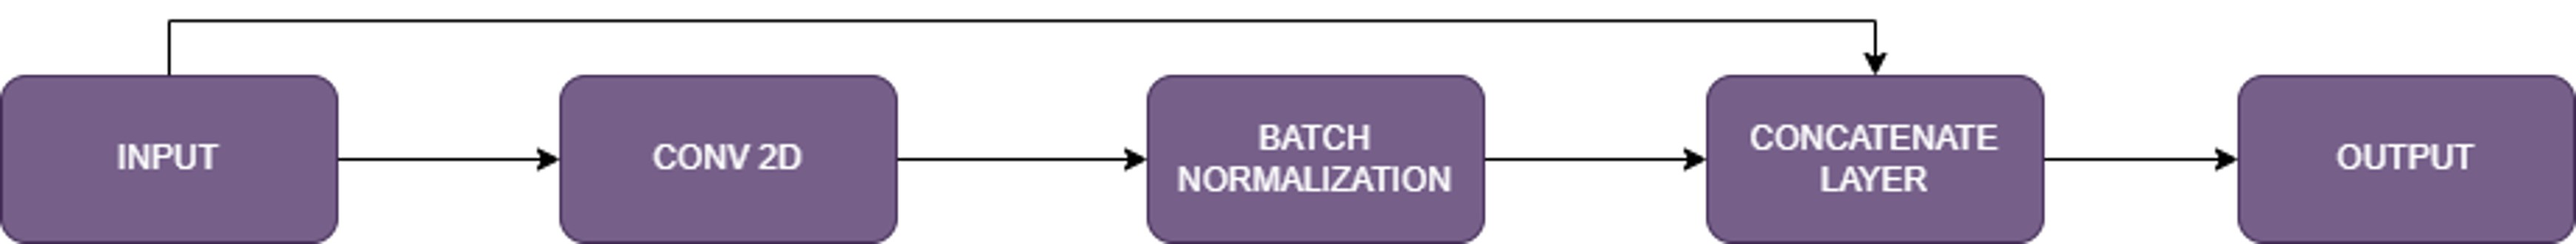
\includegraphics[width=\columnwidth,height=0.27\textheight,keepaspectratio]{paper_figures/skip_block.jpg}
\caption{Proposed SkipConnection(Concat) block.}
\label{fig:skip}
\end{figure}

\subsubsection{Global Average Pooling}
Earlier model-development records contain a parameter-heavy flattening head. The final architecture uses global average pooling. Flattening a $H\times W\times C$ tensor exposes $HWC$ values to the dense layer, whereas global average pooling exposes $C$ channel descriptors. This substantially reduces the dense-interface dimensionality. The final saved model contains 934,200 total parameters, comprising 933,720 trainable and 480 non-trainable parameters.

\begin{table*}[!t]
\centering
\caption{Layer-wise configuration of the final PlantDiseaseNet-Hybrid model.}
\label{tab:model}
\begin{tabular}{p{3.3cm}p{3.5cm}r p{5.0cm}}
\toprule
Layer & Output shape & Parameters & Operation \\
\midrule
Input & $256\times256\times3$ & 0 & RGB input \\
Inception(Add)-1 & $256\times256\times16$ & 4,032 & $3\times3$, $5\times5$, $7\times7$ + Add \\
BatchNorm + Pool-1 & $128\times128\times16$ & 64 & Normalisation and downsampling \\
Inception(Add)-2 & $128\times128\times32$ & 42,592 & Multi-scale convolution + Add \\
BatchNorm + Pool-2 & $64\times64\times32$ & 128 & Normalisation and downsampling \\
SkipConnection(Concat)-1 & $64\times64\times96$ & 100,672 & $7\times7$ + BN + Concat \\
Pool-3 & $32\times32\times96$ & 0 & Downsampling \\
SkipConnection(Concat)-2 & $32\times32\times224$ & 602,752 & $7\times7$ + BN + Concat \\
Pool-4 & $16\times16\times224$ & 0 & Downsampling \\
Global Average Pooling & 224 & 0 & Spatial aggregation \\
Dense-512 & 512 & 115,200 & ReLU \\
Dropout & 512 & 0 & Regularisation \\
Dense-128 & 128 & 65,664 & ReLU \\
Dropout & 128 & 0 & Regularisation \\
Output & 24 & 3,096 & Softmax \\
\midrule
\multicolumn{2}{r}{Total} & 934,200 & \\
\bottomrule
\end{tabular}
\end{table*}

\subsection{Training Configuration}
The experiments use TensorFlow/Keras in Kaggle GPU environments with NVIDIA Tesla T4 hardware. The final combined model uses Adam with initial learning rate 0.001, batch size 32, a maximum of 60 epochs, categorical cross-entropy, cosine warmup annealing, and early stopping with patience 12. Crop-specific notebooks preserve their recorded experiment settings where they differ.

\begin{table}[!t]
\centering
\caption{Principal training configuration.}
\label{tab:training}
\begin{tabular}{ll}
\toprule
Parameter & Value \\
\midrule
Input size & $256\times256\times3$ \\
Batch size & 32 \\
Maximum epochs & 60 \\
Optimiser & Adam \\
Initial learning rate & 0.001 \\
Scheduler & Cosine warmup annealing \\
Early stopping & Patience 12 \\
Loss & Categorical cross-entropy \\
\bottomrule
\end{tabular}
\end{table}

\subsection{Evaluation Metrics}
Accuracy, precision, recall, F1-score, specificity, and ROC--AUC are reported where available in the saved experimental records. For multi-class tasks, class-wise predictions are treated using the one-vs-rest interpretation when specificity or ROC--AUC is computed. Macro and weighted averages are not interchanged.

\section{Experimental Design}
\subsection{Primary Crop Experiments}
NB1 Wheat Hybrid, NB2 Cotton Hybrid, and NB3 PlantVillage Hybrid are dataset-specific evaluations. They are not architectural ablations because the dataset and label space change.

\subsection{Architecture Ablation}
The controlled architecture study uses the combined 24-class benchmark and compares Standard Inception, a residual CNN, Inception(Add)-only, SkipConnection(Concat)-only, and the complete hybrid. Here the word ``ablation'' refers specifically to removal or isolation of architectural components under the same task.

\subsection{Augmentation Study}
The augmentation study compares five policies on the combined task: no augmentation, LightAug, an independent LightAug repeat, CropColour, and FullAug. The purpose is to determine whether augmentation improves the task and whether stronger augmentation remains beneficial.

\subsection{SoyDisease Study}
SoyDisease is evaluated separately. The original published dataset contains 3363 images across six categories. The processed experimental subset contains 1176 images: Healthy 288, Vein Necrosis 138, Dry Leaf 230, Septoria Brown Spot 284, Root Images 10, and Bacterial Leaf Blight 226. Because the Root Images class contains only ten source images, single-split results are interpreted cautiously and five-fold validation is used for the strongest configuration.

\section{Results}
\subsection{Primary Crop Results}
\begin{table*}[!t]
\centering
\caption{Repository-verified primary crop results.}
\label{tab:primary}
\begin{tabular}{lrrrrrrr}
\toprule
Experiment & Classes & Accuracy & Precision & Recall & F1 & Specificity & Parameters \\
\midrule
NB1 Wheat Hybrid & 3 & 97.81\% & 97.82\% & 97.81\% & 97.81\% & 98.54\% & 59.78M \\
NB2 Cotton Hybrid & 6 & 53.55\% & 53.01\% & 53.55\% & 51.66\% & 90.71\% & 59.78M \\
NB3 PlantVillage Hybrid & 15 & 97.67\% & 97.68\% & 97.67\% & 97.68\% & 99.83\% & 59.78M \\
\bottomrule
\end{tabular}
\end{table*}

The crop-specific results should not be ranked directly because the datasets differ. Wheat and selected PlantVillage experiments show strong classification performance, whereas cotton is substantially harder for this implementation. The lower cotton result is retained because it is evidence of cross-domain variation rather than a value that should be removed from the study.

The Wheat experiment has an important data-quality qualification: the stored classification report records zero test support for the Wheat Healthy class. The 97.81\% overall value is therefore not interpreted as evidence of balanced three-class generalisation.

\subsection{Architecture Comparison}
\begin{table*}[!t]
\centering
\caption{Controlled architecture comparison on the combined 24-class benchmark.}
\label{tab:ablation}
\begin{tabular}{lrrrrrr}
\toprule
Model & Parameters & Accuracy & Precision & Recall & F1 & Specificity \\
\midrule
Standard Inception + GAP & 270,656 & 95.33\% & 95.34\% & 95.33\% & 95.32\% & 99.80\% \\
Residual CNN + GAP & 741,720 & \textbf{96.04\%} & 96.03\% & 96.04\% & 96.02\% & 99.83\% \\
Inception(Add)-only + GAP & 949,112 & 95.84\% & 95.84\% & 95.84\% & 95.82\% & 99.82\% \\
SkipConcat-only + GAP & 1,139,640 & 95.67\% & 95.70\% & 95.67\% & 95.67\% & 99.81\% \\
PlantDiseaseNet-Hybrid & 934,200 & 95.91\% & 95.98\% & 95.91\% & 95.91\% & 99.82\% \\
\bottomrule
\end{tabular}
\end{table*}

The residual baseline is the accuracy leader in this controlled comparison, exceeding the hybrid by 0.13 percentage points. Therefore, the paper does not claim universal accuracy superiority. The hybrid is instead characterised by its complementary fusion design and its intermediate parameter count: it is larger than Standard Inception but smaller than the SkipConcat-only variant.

\subsection{Computational Analysis}
\begin{table}[!t]
\centering
\caption{Recorded computational characteristics of the final hybrid.}
\label{tab:complexity}
\begin{tabular}{lr}
\toprule
Metric & Value \\
\midrule
Total parameters & 934,200 \\
Trainable parameters & 933,720 \\
Non-trainable parameters & 480 \\
FLOPs & 3984.7M \\
Single-image inference & 28.06 ms \\
Batch inference & 3.39 ms/image \\
\bottomrule
\end{tabular}
\end{table}

The computational measurements are hardware- and implementation-specific. The important architectural observation is that global average pooling removes the large dense-interface expansion seen in earlier flatten-based versions.

\subsection{Strategic Augmentation Results}
\begin{table*}[!t]
\centering
\caption{Recorded augmentation sensitivity study.}
\label{tab:augresults}
\begin{tabular}{p{3.2cm}p{6.2cm}rrr}
\toprule
Configuration & Policy & Accuracy & F1 & Specificity \\
\midrule
Hybrid-NoAug & No additional augmentation & 96.03\% & 96.04\% & 99.82\% \\
Hybrid-LightAug & Horizontal flip + brightness & \textbf{97.06\%} & 97.06\% & 99.87\% \\
Hybrid-LightAug-v2 & Independent LightAug repeat & 96.43\% & 96.42\% & 99.85\% \\
Hybrid-CropColour & Crop + colour transformations & 96.31\% & 96.31\% & 99.84\% \\
Hybrid-FullAug & Full recorded transformation set & 95.91\% & 95.91\% & 99.82\% \\
\bottomrule
\end{tabular}
\end{table*}

LightAug provides the best recorded result, improving the no-augmentation accuracy by 1.03 percentage points. The independent LightAug-v2 run records 96.43\%, showing run-to-run variation. FullAug does not improve performance and returns to 95.91\%. The evidence therefore supports selective rather than indiscriminate augmentation.

\subsection{PlantVillage--Wheat Extended Benchmark}
The original draft records an 18-class PlantVillage--Wheat benchmark. The no-augmentation configuration records 99.12\% accuracy, 99.13\% precision, 99.12\% recall, 99.12\% F1, and macro AUC 1.0000. The LightAug configuration records 99.46\% accuracy. These values are retained as original-draft benchmark results and are not used to rank the 24-class architecture variants because the tasks differ.

\subsection{SoyDisease Results}
\begin{table}[!t]
\centering
\caption{Recorded SoyDisease experiments.}
\label{tab:soy}
\begin{tabular}{lrrr}
\toprule
Experiment & Accuracy & Precision & F1 \\
\midrule
EXP-1 & 100.00\% & 1.000 & 1.000 \\
EXP-2 & 100.00\% & 1.000 & 1.000 \\
EXP-3 & 85.88\% & 0.905 & 0.857 \\
EXP-4 & 99.44\% & 0.995 & 0.994 \\
\bottomrule
\end{tabular}
\end{table}

EXP-1 and EXP-2 reach 100\% on their recorded single split, but those values are statistically fragile because the processed dataset contains only ten Root Images samples. EXP-4 records 99.44\% on its held-out evaluation and 99.57\% $\pm$ 0.85\% across five-fold validation. The fold accuracies are 100.00\%, 100.00\%, 97.87\%, 100.00\%, and 100.00\%. The five-fold result is therefore the preferred soybean estimate.

\section{Discussion}
The proposed architecture is best understood as a deliberate allocation of fusion operations. Addition is used at the high-resolution multi-scale stage because it prevents branch-wise channel multiplication. Concatenation is used after downsampling because preserving both the incoming and transformed features is useful and more computationally manageable at lower spatial resolutions.

The controlled architecture results show that this design is not automatically the most accurate. ResNet reaches 96.04\%, compared with 95.91\% for the complete hybrid. This is not a failure of the experiment; it is an important negative comparison that prevents overclaiming. Standard Inception has fewer parameters, while SkipConcat-only has more parameters without exceeding the complete hybrid. The result suggests that the hybrid occupies a middle point in the accuracy--capacity trade-off.

The augmentation study gives a similarly nuanced result. LightAug performs best, while FullAug does not. This indicates that transformations should be selected according to plausible nuisance variation and validated experimentally. The LightAug repeat also demonstrates that one training run should not be treated as an exact deterministic estimate of the augmentation gain.

The primary crop experiments demonstrate domain sensitivity. The large difference between PlantVillage/wheat performance and cotton performance means that a strong benchmark result should not be described as universal cross-crop robustness. The cotton result is retained specifically to make this limitation visible.

SoyDisease further demonstrates the importance of evaluation protocol. The small Root Images class makes single-split scores unstable, and the five-fold result provides a more informative summary. This is why 99.57\% $\pm$ 0.85\% is preferred over the 100\% single-split values.

Finally, the parameter discrepancy across the project is explained by architecture generation. Earlier flatten-based implementations produced approximately 59.8M parameters. The final global-average-pooling implementation contains 934,200 total parameters. These numbers belong to different implementations and must not be mixed in a single complexity claim.

\section{Limitations}
The datasets differ in size, class balance, image acquisition, and disease semantics. Consequently, crop-specific accuracies are not directly comparable as a single ranking. The Wheat test report has zero support for the Healthy class and therefore weakens the interpretation of its overall accuracy. Cotton remains a difficult setting for the current implementation. Some augmentation-study values are retained from the project experiment record without an independently exported small metric file for every augmentation notebook; they should be matched to the saved notebook outputs before final journal submission. Finally, inference measurements depend on the recorded hardware and software environment.

\section{Conclusion and Future Directions}
This work presented PlantDiseaseNet-Hybrid, a custom CNN that combines Inception(Add) and SkipConnection(Concat) as complementary feature-fusion mechanisms. Addition provides compact multi-scale integration, while concatenation preserves earlier features. Global average pooling controls the classifier-head dimensionality and resolves the parameter expansion observed in earlier flatten-based implementations.

The evidence supports a measured conclusion. The hybrid achieves strong performance on selected wheat and PlantVillage settings and reaches 95.91\% on the controlled 24-class benchmark. It does not outperform the residual baseline, and cotton remains substantially more difficult. The augmentation study identifies LightAug as the best recorded policy at 97.06\%, while the SoyDisease study records 99.57\% $\pm$ 0.85\% five-fold accuracy for its strongest configuration. Future work should evaluate repeated seeds, larger field datasets, domain shift, class-balanced training, explainability, attention mechanisms, and edge deployment.

\section*{Data Availability}
PlantVillage and the wheat resources are publicly available. The cotton dataset is publicly available through the Cotton Plant Disease dataset record attributed to Dhamodharan. The India SoyDisease dataset is publicly available through Mendeley Data. The processed subsets and class mappings used in this study are documented in the paper-aligned repository.

\section*{Code Availability}
The paper-aligned repository contains the executed research notebooks, figures, results CSV, dataset provenance information, and manuscript source. The notebooks are retained as executed research records and are not executed during manuscript preparation.

\section*{Conflict of Interest}
The authors declare no conflict of interest.

\section*{Funding}
No external funding was received for this work.

\begin{thebibliography}{99}
\bibitem[Hughes and Salathé(2015)]{hughes2015} D. P. Hughes and M. Salathé, ``An open access repository of images on plant health to enable the development of mobile disease diagnostics,'' arXiv:1511.08060, 2015.
\bibitem[Mohanty et al.(2016)]{mohanty2016} S. P. Mohanty, D. P. Hughes, and M. Salathé, ``Using deep learning for image-based plant disease detection,'' \textit{Frontiers in Plant Science}, 7, 1419, 2016. doi:10.3389/fpls.2016.01419.
\bibitem[Szegedy et al.(2015)]{szegedy2015} C. Szegedy, W. Liu, Y. Jia, P. Sermanet, S. Reed, D. Anguelov, D. Erhan, V. Vanhoucke, and A. Rabinovich, ``Going deeper with convolutions,'' \textit{Proceedings of the IEEE Conference on Computer Vision and Pattern Recognition}, 1--9, 2015. doi:10.1109/CVPR.2015.7298594.
\bibitem[He et al.(2016)]{he2016} K. He, X. Zhang, S. Ren, and J. Sun, ``Deep residual learning for image recognition,'' \textit{Proceedings of the IEEE Conference on Computer Vision and Pattern Recognition}, 770--778, 2016. doi:10.1109/CVPR.2016.90.
\bibitem[Huang et al.(2017)]{huang2017} G. Huang, Z. Liu, L. van der Maaten, and K. Q. Weinberger, ``Densely connected convolutional networks,'' \textit{Proceedings of the IEEE Conference on Computer Vision and Pattern Recognition}, 4700--4708, 2017.
\bibitem[Too et al.(2019)]{too2019} E. C. Too, L. Yujian, S. Njuki, and Y. Yingchun, ``A comparative study of fine-tuning deep learning models for plant disease identification,'' \textit{Computers and Electronics in Agriculture}, 161, 272--279, 2019. doi:10.1016/j.compag.2018.03.032.
\bibitem[Atila et al.(2021)]{atila2021} Ü. Atila, M. Uçar, K. Akyol, and E. Uçar, ``Plant leaf disease classification using EfficientNet deep learning model,'' \textit{Ecological Informatics}, 61, 101182, 2021. doi:10.1016/j.ecoinf.2020.101182.
\bibitem[Safarijalal et al.(2022)]{safarijalal2022} B. Safarijalal, Y. Alborzi, and E. Najafi, ``Automated wheat disease detection using a ROS-based autonomous guided UAV,'' Research Square, 2022. doi:10.21203/rs.3.rs-1251771/v1.
\bibitem[Long et al.(2023)]{long2023} M. Long, M. Hartley, R. J. Morris, and J. K. M. Brown, ``Classification of wheat diseases using deep learning networks with field and glasshouse images,'' \textit{Plant Pathology}, 72(3), 536--547, 2023. doi:10.1111/ppa.13684.
\bibitem[Kotwal et al.(2024)]{kotwal2024} J. Kotwal, R. Kashyap, and M. S. Pathan, ``An India soyabean dataset for identification and classification of diseases using computer-vision algorithms,'' \textit{Data in Brief}, 53, 110216, 2024. doi:10.1016/j.dib.2024.110216.
\bibitem[Johri et al.(2024)]{cotton2024} P. Johri, S. Kim, K. Dixit, P. Sharma, B. Kakkar, Y. Kumar, J. Shafi, and M. F. Ijaz, ``Advanced deep transfer learning techniques for efficient detection of cotton plant diseases,'' \textit{Frontiers in Plant Science}, 15, 1441117, 2024. doi:10.3389/fpls.2024.1441117.
\bibitem[Mhala et al.(2025)]{mhala2025} P. Mhala, A. Bilandani, and S. Sharma, ``Enhancing crop productivity with fine-tuned deep convolution neural network for potato leaf disease detection,'' \textit{Expert Systems with Applications}, 267, 126066, 2025. doi:10.1016/j.eswa.2024.126066.
\bibitem[Saleem et al.(2019)]{saleem2019} M. H. Saleem, J. Potgieter, and K. M. Arif, ``Plant disease detection and classification by deep learning,'' \textit{Plants}, 8(11), 468, 2019. doi:10.3390/plants8110468.
\end{thebibliography}
\end{document}
